\documentclass[a4paper,11pt]{book}
\usepackage{fullpage}
\usepackage{amsmath}
\usepackage{amssymb}
\usepackage{amstext}
\usepackage{array}

\usepackage{tikz-qtree,tikz-qtree-compat}
\usepackage{tikz}
\usetikzlibrary{shapes.geometric}
\usetikzlibrary{shapes.multipart}
\usetikzlibrary{shadows}
\usetikzlibrary{positioning}
\usetikzlibrary{trees}
\usetikzlibrary{arrows}

\usepackage{algorithm}
\usepackage{algorithmicx,algpseudocode}

\newlength{\OUmatrixSepWidth}
\newcommand{\OUsetMatrixSepWidth}[1]{%
	\settowidth{\OUmatrixSepWidth}{#1}%
}


\title{Algorithm Design and Analysis (ECS 122A)\\Study Guide}
\author{Davis Computer Science Club\\
	Tutoring Committee
}
\date{Spring Quarter 2015}



\begin{document}

\makeatletter
\begin{titlepage}
	
\noindent \rule{\textwidth}{1pt}

\vspace{1cm}

\noindent {\LARGE \bfseries \@title}

\vspace{1cm}

\noindent \rule{\textwidth}{1pt}

\vspace{1cm}

\noindent	{\Large \@author }

\par\vspace*{\fill}
\begin{flushright}
	Spring Quarter 2015
\end{flushright}
\end{titlepage}

\tableofcontents
\newpage

% 
% ASYMPTOTIC NOTATION
%
\chapter{Asymptotic Notation}
\newpage
% Big O
\section{O-Notation (Big O)}

\subsection*{Notation}
$$f(n) \in O(g(n))$$

\subsection*{Formal Definition}
For a given function $g(n)$, $O(g(n))$ is the set of functions for which there exists positive constants $c$ and $n_0$ such that $0 \leq f(n) \leq c \cdot g(n)$ for all $n \geq n_0$.
$$
O(g(n)) = \{ f(n) : \exists \text{ } c, n_0 \text{ s.t. } 0 \leq f(n) \leq c \cdot g(n) \text{ } \forall \text{ } n \geq n_0 \}
$$

\subsection*{Informal Definition}
The function $g(n)$ is an asymptotic upper bound for the function $f(n)$ if there exists constants $c$ and $n_0$ such that $0 \leq f(n) \leq c \cdot g(n)$ for $n \geq n_0$.\\\\
Another way to perceive Big O notation is that for $f(n) \in O(g(n))$, the function $f$'s asymptotic\footnote{Asymptotic: As given variable approaches infinity.} growth is no faster than that of function $g$'s.

\subsection*{Limit Definition}
$$ 
\lim\limits_{n \to \infty} \frac{f(n)}{g(n)} < \infty
$$

\subsection{Example}
\textbf{Prove that asymptotic upper bound of $f(n) = 2n+10$ is $g(n) = n^2$}.
\begin{eqnarray*}
	0 \leq f(n) &\leq& c \cdot g(n) \text{ for } n \geq n_0\\
	0 \leq 2n + 10 &\leq& c \cdot n^2 \text{ for } n \geq n_0
\end{eqnarray*}
Arbitrarily choose $c$ and $n_0$ values. Simplest is to turn one of the variables into the value $1$ and solve. For this example, we will assign the value 1 to $n_0$.
\begin{eqnarray*}
	0 \leq 2n + 10 &\leq& c \cdot n^2 \text{ for } n \geq 1\\
	2(1) + 10 &\leq& c \cdot (1)^2\\
	12 &\leq& c
\end{eqnarray*}
By picking $n_0 = 1$ and $c = 12$, the inequality of $2n+10 \leq 12n^2$ will hold true for all $n \geq 1$. Since there exists a constant $c$ and $n_0$ that fulfill this inequality, we have proven that $f(n) = 2n+10 = O(n^2)$.
\newpage

% Little O
\section{o-Notation (Little O)}

\subsection*{Notation}
$$
f(n) \in o(g(n))
$$

\subsection*{Formal Definition}
For a given function $g(n)$, $o(g(n))$ is the set  of functions for which every positive constant $c > 0$, there exists a constant $n_0 > 0$ such that $0 \leq f(n) \leq c \cdot g(n)$ for all $n \geq n_0$.
$$
o(g(n)) = \{ f(n) : \exists \text{ } n_0 \text{ s.t. } 0 \leq f(n) \leq c \cdot g(n) \text{ } \forall \text{ } n \geq n_0, c \geq 0 \}
$$

\subsection*{Informal Definition}
The function g(n) is an upper bound that is not asymptotically tight. For all positive constant values of $c$, there must exists a constant $n_0$ such that $0 \leq f(n) \leq c \cdot g(n)$ for all $n \geq n_0$. The value of $n_0$ may not depend on n, but may depend on $c$.\\\\
Another way to perceive Little O notation is that for $f(n) \in o(g(n))$, the function $f$'s asymptotic growth is strictly less than that of the function $g$'s. In this sense, Little O can be seen as a ``stronger" bound in comparison to Big O. By proving that a function is an element of Little O, it also proves that the function is an element of Big O.

\subsection*{Limit Definition}
$$
\lim\limits_{n\to\infty} \frac{f(n)}{g(n)} = 0
$$

\subsection{Example}
\textbf{Prove that $f(n) = 2n$ has an upper bound $o(n^2)$.}
\begin{eqnarray*}
	0 \leq c \cdot g(n) &\leq& f(n) \text{ for } n \geq n_0\\
	0 \leq c \cdot 2n &\leq& n^2 \text{ for } n \geq n_0\\
	2c &\leq& n \text{ for } n \geq n_0\\
	2c &\leq& n_0
\end{eqnarray*}
For Little O to hold true, the inequality needs to hold true for all $c > 0$ and for all $n > n_0$. From simplifying the inequality, we assert that the inequality will hold true as long as the value of $n_0$ is twice the value of $c$. Given that they are both constants, then there exists a constant value of $n_0$ for all positive constant $c$ that fulfill this inequality.\\\\
Another method to solve this problem is to use the limit definition.
\begin{eqnarray*}
	&\lim\limits_{n\to\infty}& \frac{2n}{n^2}\\
	&\lim\limits_{n\to\infty}& \frac{2}{n} = 0	
\end{eqnarray*}

\newpage

\subsection{Example}
\textbf{Prove that $f(n) = 2n^2$ does not have the upper bound $o(n^2)$.}
\begin{eqnarray*}
	0 \leq c \cdot g(n) &\leq& f(n) \text{ for } n \geq n_0\\
	0 \leq c \cdot 2n^2 &\leq& n^2 \text{ for } n \geq n_0\\
	2c &\leq& 1\text{ for } n \geq n_0
\end{eqnarray*}
For a function to have the Little O bound, the inequality must hold true for all positive $c$. However, simplification of the inequality asserts that the inequality will only hold true for all $c < \frac{1}{2}$. Therefore, $f(n) = 2n^2$ does not have the upper bound $o(n^2)$.
\newpage

% Big Omega
\section{$\Omega$-Notation (Big Omega)}

\subsection*{Notation}
$$
f(n) \in \Omega(g(n))
$$

\subsection*{Formal Definition}
For a given function $g(n)$, $\Omega(g(n))$ is the set of functions for which there exists positive constants $c$ and $n_0$ such that $0 \leq c \cdot g(n) \leq f(n)$ for all $n \geq n_0$.
$$
\Omega(g(n)) = \{ f(n) : \exists \text{ } c, n_0 \text{ s.t. } 0 \leq c \cdot g(n) \leq f(n) \text{ } \forall \text{ } n \geq n_0 \}
$$

\subsection*{Informal Definition}
The function $g(n)$ is an asymptotic lower bound for the function $f(n)$ if there exists constants $c$ and $n_0$ such that $0 \leq c \cdot g(n) \leq f(n)$ for $n \geq n_0$.

\subsection*{Limit Definition}
$$
\lim\limits_{n \to \infty} \frac{f(n)}{g(n)} > 0
$$
\newpage

% Little Omega
\input{asymptotic/little-omega.tex}
\newpage

% Theta
\section{$\Theta$-notation (Big Theta)}

\subsection*{Notation}
$$
f(n) \in \Theta(g(n))
$$

\subsection*{Formal Definition}
For a given function $g(n)$, $\Theta(g(n))$ is the set of functions for which there exists positive constants $c_1$, $c_2$, and $n_0$ such that $0 \leq c_1 \cdot g(n) \leq f(n) \leq c_2 \cdot g(n)$ for all $n \geq n_0$.
$$
\Theta(g(n)) = \{ f(n) : \exists \text{ } c_1, c_2, n_0 \text{ s.t. } 0 \leq c_1 \cdot g(n) \leq f(n) \leq c_2 \cdot g(n) \text{ } \forall \text{ } n \geq n_0 \}
$$

\subsection*{Informal Definition}
The function g(n) is an asymptotic tight bound for the function f(n) if there exists constants $c_1$, $c_2$, and $n_0$ such that $0 \leq c_1 \cdot g(n) \leq f(n) \leq c_2 \cdot g(n)$ for $n \geq n_0$.\\\\
Big theta implies that $f(n) = O(g(n))$ and $f(n) = \Omega(g(n))$.

\subsection*{Limit Definition}
$$
\lim\limits_{n\to\infty} \frac{f(n)}{g(n)} \in \mathbb{R}_{>0}
$$
\newpage

%
% RECURRENCE RELATIONS
%
\section{Recurrence Relations}
A recurrence relation is an equation that recursively defines a sequence of values. After the initial terms are given, each subsequent term is defined as a function of the previous terms.

\subsection{Fibonacci}
Fibonacci is an example of a recurrence relation.
$$
F_n = \begin{cases}
	F_{n-1} + F_{n-2}, &  n \geq 2\\
	1, & n = 1\\
	0, & n = 0
\end{cases}
$$
The first two terms are defined while the subsequent terms are a function of the two previous.

\subsection{Solving Recurrence Relations with Induction}

\subsubsection{Example}
\textbf{Prove that the following systems of equations has the solution $T(n) = n \cdot lg(n)$.}
$$
T(n) \begin{cases}
	2T(\frac{n}{2}) + n, & n = 2^k \mbox{ for } k > 1\\
	2, & n = 2
\end{cases}
$$
\textbf{Basis}
\begin{eqnarray*}
T(2) &=& (2) \cdot lg(2)\\
	&=& 2 \cdot 1\\
	&=& 2
\end{eqnarray*}
\textbf{Inductive Hypothesis}\\
Assume that $T(n) = n \cdot lg(n)$ holds true for all $n = 2^k$.\\\\
\textbf{Inductive Step}
\begin{align*}
T(n)	&=	2T(\frac{n}{2}) + n						&& \text{Base equation}\\
		&= 	2T(\frac{2^{k+1}}{2}) + 2^{k+1}			&& \text{Substitute n with } 2^{k+1}\\
		&= 	2T(2^{k}) + 2^{k+1}						&& \text{Simplify parameters to function T(...)}\\
		&=	2(2^k \cdot lg(2^k)) + 2^{k+1}			&& \text{Inductive hypothesis}\\
		&=	2^{k+1} \left[ lg(2^k) + 1 \right]		&& \text{Distributive property}\\
		&=  2^{k+1} \left[ lg(2^k) + lg(2) \right]  && \text{Logarithmic identity}\\
		&= 	2^{k+1} \cdot lg(2^k \cdot 2)			&& \text{Logarithmic identity}\\
		&=  2^{k+1} \cdot lg(2^{k+1})				&& \text{Exponent property}\\
		&											&& \text{Q.E.D}
\end{align*}

\subsubsection{Example}
\textbf{Prove that the following systems of equations has the solution $T(n) = 2F(n) - 1$ where $F(n) = F(n-1) + F(n-2)$.}
$$
T(n) \begin{cases}
T(n-1) + T(n-2) + 1, & \mbox{if } n \geq 2\\
0, & \mbox{if } n = \{0,1\}
\end{cases}
$$
\textbf{Basis}
\begin{eqnarray*}
	T(0) &=& 1
\end{eqnarray*}
\textbf{Inductive Hypothesis}\\
Assume that $T(n) = F(n) - 1$ is true for all $n = k$.\\
\textbf{Inductive Step}
\begin{align*}
	T(n) 	&= T(n-1) + T(n-2) + 1					&& \text{Base equation}\\
	T(k+1) 	&= T((k+1) - 1) + T((k+1) - 2) + 1 		&& \text{Substitute n with k+1}\\
			&= T(k) + T(k-1) + 1					&& \text{Simplify parameters to function T(...)}\\
			&= (2F(k) - 1) + (2F(k-1) - 1) + 1		&& \text{Inductive hypothesis}\\
			&= 2F(k) + 2F(k-1) - 1					&& \text{Simplify equation}\\
			&= 2(F(k) + F(k-1)) - 1					&& \text{Distributive property}\\
			&= 2(F(k+1)) - 1						&& \text{Definition of function: } F(k+1) = F(k) + F(k-1)\\
			&= 2F(k+1) - 1							&& \text{Simplify}\\
			&										&& \text{Q.E.D}
\end{align*}

% Divide-and-Conquer Recurrence

% Master Theorem

%
% DIVIDE AND CONQUER
%
\chapter{Divide and Conquer Algorithms}
\newpage



%
% GREEDY ALGORITHM
%
\chapter{Greedy Algorithm}
\newpage

\section{Properties}

\subsection*{Greedy Choice}
A globally optimal solution can be arrived at by making a locally optimal (greedy) choice.

\subsection*{Optimal Substructure Property}
An optimal solution to the problem contains within it optimal solution to the subproblems.

\newpage


\section{Case Study: Activity-Selection}

\subsection{Formal Problem Statement}
Assume there exists $n$ activities, each with a start time $s_i$ and finish time $f_i$. Two activities $i$ and $j$ are said to be non-conflicting if $s_i \geq f_j$ or $s_j \geq f_i$. The objective is to find the maximum solution set of non-conflicting activities.

\subsection{Informal Problem Statement}
Given $n$ activities and their respective start ($s_i$) and finish ($f_i$) times, find the maximum number of activities that can be performed.

\subsection{Greedy Choice}
Choose the next activity with a start time greater than or equal to the previous activity's finish time and has the next smallest finish time.

\subsection{Steps}
\begin{enumerate}
	\item Sort the activities according to their finish times. 
	\item Select the first activity from the sorted list.
	\item Repeat this process for the remaining activities with the condition that the start time of subsequent activities are greater than or equal to the preceding activity's finish time. 
\end{enumerate}

\subsection{Pseudocode}
\begin{algorithm}
\begin{algorithmic}[1]
\Procedure{ActivitySelection}{A}
	\State Sort(A) \Comment{Sort by finish times}\\
	\State Let F be the set of finish times corresponding to the sorted list A
	\State Let B be the set of start times correspdonding to the sorted list A\\
	\State S = \{ A[1] \}
	\State f = $F_0$\\
	\For{i=2 \textbf{to} n}
		\If{$F_i \geq $ f}
			\State S $\cup \text{ } \{$ A[i] $\}$
			\State f = $F_i$
		\EndIf	
	\EndFor
\EndProcedure
\end{algorithmic}
\end{algorithm}
\newpage

\section{Case Study: Huffman Coding}

\subsection*{Formal Problem Statement}
Let A be defined as the set of alphabets. ( $A = \{ a_0, a_1, a_2, ..., a_n \}$ )\\
Let W be defined as the set of weights for which $w_i = \text{Weight}(a_i)$.  ($W = \{ w_0, w_1, w_2, ..., w_n \}$)
Let C be defined as the set of (binary) codewords for which $c_i = \text{CodeWord}(a_i)$.\\\\
Assume there exists $n$ alphabets, each with a weight $w_i$. Find and define the codewords $c_i$ for each respective alphabet $a_i$ such that $\sum\limits_{i=0}^{n} w_i \cdot length(c_i)$ is the smallest possible.

\subsection*{Informal Problem Statement}
Given a set of symbols and their weights (probabilities), find a prefix-free binary code with minimum expected codeword length.

\subsection*{Greedy Choice}
Choose the two alphabets with the lowest weight. 

\subsection*{Steps}
\begin{enumerate}
	\item Pick two letters $x$ and $y$ from the alphabet A with the lowest frequencies or weight $w_i$.
	\item Create a subtree with $x$ and $y$ as leaves. We will define the root as $z$.
	\item The frequency or weight of node $z$ will be define as $w_z = w_x + w_y$.
	\item Remove $x$ and $y$ from alphabet.\\
		$ A^\prime = A - \{ x, y \}$
	\item Insert $z$ into the alphabet.\\
		$ A^\prime = A + \{ z \} $
	\item Repeat this process until the set of alphabets $A$ consists of only one alphabet.
\end{enumerate}

\subsection*{Complexity}
$$O(n \cdot lg(n))$$
Total = $O(n \cdot lg(n)) + \Theta(n)$. Cost to sort alphabet by weight and cost to iterate through all alphabets.

\newpage

\subsection{Example}
\textbf{Let $A = \{ a, b, c, d, e \}$ and $W = \{ 30, 16, 6, 15, 35 \}$. Find their corresponding Huffman codes.}

\subsubsection*{Merge $c$ and $d$}
\begin{minipage}{0.35\linewidth}
	\flushleft
	\begin{tabular}{| c | c |}
		\hline
		Alphabet	&	Weight\\
		\hline
		e			&	35\\
		\hline
		a			&	30\\
		\hline
		b			&	16\\
		\hline
		d			&	15\\
		\hline
		c			&	6\\
		\hline
	\end{tabular}
\end{minipage}
\qquad
\begin{minipage}{0.65\linewidth}
	\centering
	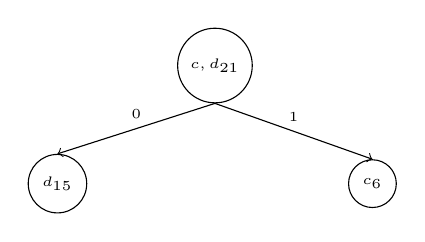
\begin{tikzpicture}[level/.style={sibling distance=40mm/#1}]
	\node [circle,draw] {\tiny$c,d_{21}$}
	child {
		node [circle,draw] {\tiny$d_{15}$}
		edge from parent [->] node [above] {\tiny 0}
	}
	child {
		node [circle,draw] {\tiny$c_6 $}
		edge from parent [->] node [above] {\tiny 1}
	};
	\end{tikzpicture}
\end{minipage}


\subsubsection*{Merge $c,d$ and $b$}
	\begin{minipage}{0.35\linewidth}
		\flushleft
		\begin{tabular}{| c | c |}
			\hline
			Alphabet	&	Weight\\
			\hline
			e			&	35\\
			\hline
			a			&	30\\
			\hline
			c,d			&	21\\
			\hline
			b			&	16\\
			\hline
		\end{tabular}
	\end{minipage}
	\qquad
\begin{minipage}{0.65\linewidth}
	\centering
	\begin{tikzpicture}[level/.style={sibling distance=60mm/#1}]
	\node [circle,draw] {\tiny$b,c,d_{37}$}
	child {
		node [circle,draw] {\tiny$c,d_{21}$}
		child {
			node [circle,draw] {\tiny$d_{15}$}
			edge from parent [->] node [above] {\tiny 0}
		}
		child {
			node [circle, draw] {\tiny$c_{6}$}
			edge from parent [->] node [above] {\tiny 1}
		}
		edge from parent [->] node [above] {\tiny 0}
	}
	child {
		node [circle,draw] {\tiny$b_{16} $}
		edge from parent [->] node [above] {\tiny 1}
	};
	\end{tikzpicture}
\end{minipage}

\subsubsection*{Merge $e$ and $a$}
\begin{minipage}{0.35\linewidth}
\flushleft
	\begin{tabular}{| c | c |}
		\hline
		Alphabet	&	Weight\\
		\hline
		b,c,d			&	37\\
		\hline
		e			&	35\\
		\hline
		a			&	30\\
		\hline
	\end{tabular}
\end{minipage}
\qquad
\begin{minipage}{0.30\linewidth}
	\centering
	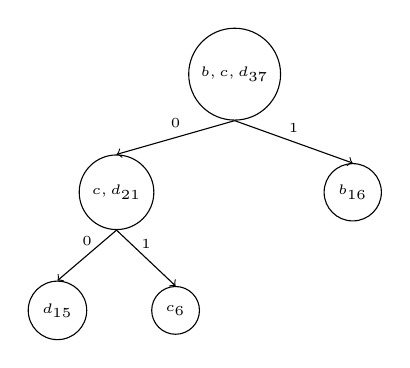
\begin{tikzpicture}[level/.style={sibling distance=30mm/#1}]
	\node [circle,draw] {\tiny$b,c,d_{37}$}
	child {
		node [circle,draw] {\tiny$c,d_{21}$}
		child {
			node [circle,draw] {\tiny$d_{15}$}
			edge from parent [->] node [above] {\tiny 0}
		}
		child {
			node [circle, draw] {\tiny$c_{6}$}
			edge from parent [->] node [above] {\tiny 1}
		}
		edge from parent [->] node [above] {\tiny 0}
	}
	child {
		node [circle,draw] {\tiny$b_{16} $}
		edge from parent [->] node [above] {\tiny 1}
	};
	\end{tikzpicture}
\end{minipage}
\begin{minipage}{0.30\linewidth}
	\centering
	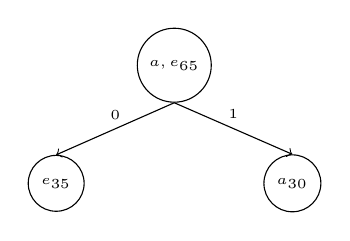
\begin{tikzpicture}[level/.style={sibling distance=30mm/#1}]
	\node [circle,draw] {\tiny$a,e_{65}$}
	child {
		node [circle,draw] {\tiny$e_{35}$}
		edge from parent [->] node [above] {\tiny 0}
	}
	child {
		node [circle,draw] {\tiny$a_{30} $}
		edge from parent [->] node [above] {\tiny 1}
	};
	\end{tikzpicture}
\end{minipage}


\subsubsection*{Merge $a,b,c,d$ and $e$}
\begin{minipage}{0.35\linewidth}
	\flushleft
	\begin{tabular}{| c | c |}
		\hline
		Alphabet	&	Weight\\
		\hline
		a,e			&	65\\
		\hline
		b,c,d		&	37\\
		\hline
	\end{tabular}
\end{minipage}
\qquad
\begin{minipage}{0.65\linewidth}
\centering
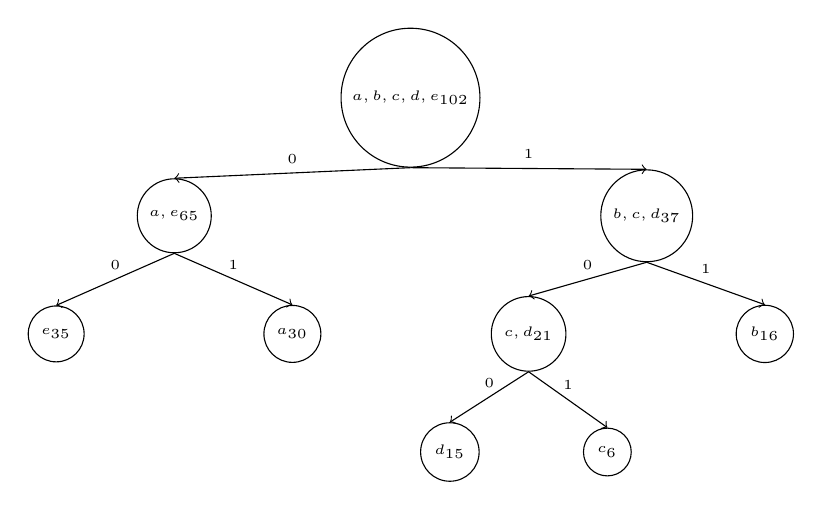
\begin{tikzpicture}[level/.style={sibling distance=60mm/#1}]
	\node [circle,draw] {\tiny$a,b,c,d,e_{102}$}
	child {
		node [circle,draw] {\tiny$a,e_{65}$}
		child {
			node [circle,draw] {\tiny$e_{35}$}
			edge from parent [->] node [above] {\tiny 0}
		}
		child {
			node [circle, draw] {\tiny$a_{30}$}
			edge from parent [->] node [above] {\tiny 1}
		}
		edge from parent [->] node [above] {\tiny 0}
	}
	child {
		node [circle,draw] {\tiny$b,c,d_{37} $}
		child {
			node [circle,draw] {\tiny $c,d_{21}$ }
			child {
				node [circle, draw] {\tiny $d_{15}$ }
				edge from parent [->] node [above] {\tiny 0}
			}
			child {
				node [circle,draw] {\tiny $c_6$}
				edge from parent [->] node [above] {\tiny 1}
			}
			edge from parent [->] node [above] {\tiny 0}
		}
		child {
			node [circle, draw] {\tiny $b_{16}$}
			edge from parent [->] node [above] {\tiny 1}
		}
		edge from parent [->] node [above] {\tiny 1}
	};
\end{tikzpicture}
\end{minipage}

\subsubsection*{Solution}

\begin{table}[H]
	\centering
	\begin{tabular}{| c | c | c |}
		\hline
		Alphabet	&	Weight	&	Codeword\\
		\hline
		e			&	35		&	00\\
		\hline
		a			&	30		&	01\\
		\hline
		b			&	16		&	11\\
		\hline
		d			&	15		&	100\\
		\hline
		e			&	6		&	101\\
		\hline
	\end{tabular}
\end{table}


\newpage

% Move to graph theory
%\section{Case Study: Minimum Spanning Tree}
%\newpage

%
% DYNAMMIC PROGRAMMING
%
\chapter{Dynamic Programming}
\newpage

\section{Case Study: Rod Cutting}
\newpage

\section{Case Study: Matrix Chain Multiplication}

\subsection*{Problem Statement}
Given a sequence of matrices $A_1, A_2, ... A_n$ with order $p_{i-1} \times p_i$, find the ordering for the product of $A_1 \times A_2 \times A_3 ... \times A_n$ such that it minimizes the number of scalar multiplications.

\subsection*{Important}
The matrix is 1-indexed while the sequence for the order of matrices is 0-indexed.

\subsection*{Steps}
\begin{enumerate}
	\item Given the orders of the matrices, create a matrix $m$ and a matrix $s$ of order $(n-1) \times (n-1)$.
	\item Zero out the main diagonal ($m[i,i] = 0$ and $s[i,i] = 0$).
	\item Each iteration creates a new diagonal that builds the upper right triangle of the $m$ and $s$ matrix.
	\item Start from the $i = 1$ and build down the diagonal.
	\item For each diagonal:
	\begin{enumerate}
		\item For each cell on the diagonal, find the minimum such that:\\
			$m[i,j] = \min\limits_{i\leq k < j} \{ m[i,k] + m[k+1,j] + p_{i-1}p_kp_j \}$. 
		\item $s[i,j]$ will be the $k$ that attains the minimum value of $m[i,j]$.
	\end{enumerate}
	\item A more visual method and informal method for each diagonal (Same as Step 4):
	\begin{enumerate}
		\item For a given cell we are trying to calculate, we will denote it as $m[i,j]$.
		\item Imagine that there exists a sliding window of size $i + j$ number of cells that curves down at $m[i,j]$.
		\item The end points of the sliding window are the left cell $(m[i,k])$ and the bottom cell $(m[k+1,j])$.
		\item Set the left cell as a cell on the main diagonal and on the same row as the cell we are trying to calculate. 
		\item Based on the constraint, this will also set the bottom cell is immediately below the current cell we are trying to calculate.
		\item Two of the orders are constant -- $p_{i-1}$ and $p_j$. The only order that changes is $p_k$ and $k$ can be easily determined by the column index of the left cell. From that you can calculate the product of orders $p_{i-1}p_k p_j$.
		\item Sum the value of the left cell, right cell, and the product of orders.
		\item Slide the window by increasing the column index in the left cell. Based on the sliding window constraint, the row index of the bottom cell must increase. Repeat steps 6a--6h until the entire sliding window is on row $j$ (This also means that the left cell is $m[i,j]$).
		\item The minimum of all these calculated values will be the value of $m[i,j]$. The left cell that achieved the minimum value will have its column index be the value of $s[i,j]$.
	\end{enumerate}
\end{enumerate}

\subsection*{Parenthesizing Based on $s$ Matrix}
\begin{enumerate}
	\item Start from the upper-right corner $(i = 1, j = n)$.
	\item Split into a binary tree and wrap the root with a pair of parentheses.
	\begin{itemize}
		\item The left will repeat this process, but from $i = i$ and $j = s[i,j]$.
		\item The right will repeat this process, but from $i= s[i,j] + 1$ and $j = j$.
	\end{itemize}
	\item Whenever $i = j$, then the print $A_i$.
\end{enumerate}
\subsection*{Complexity}
$$
\text{Time: } O(n^3)
$$
$$
\text{Space: } O(n^2)
$$

\subsection{Example}
\textbf{Let A be defined as the sequence $\{ A_1, A_2, A_3, A_4 \}$ and their orders\\ P = \{ 10, 100, 5, 50, 1  \}. Find the optimal parenthesization.}

\subsubsection*{Initialization}
\begin{minipage}{0.5\linewidth}
	$$
	m\text{-table}=
	\begin{bmatrix}
	0	&		&		&		&		\\
	&	0	&		&		&		\\
	&		&	0	&		&			\\			
	&		&		&	0	&		\\
	&		&		&		&	0	
	\end{bmatrix}
	$$
\end{minipage}
\begin{minipage}{0.5\linewidth}
$$
s\text{-table}=
\begin{bmatrix}
0	&		&		&		&		\\
&	0	&		&		&		\\
&		&	0	&		&			\\			
&		&		&	0	&		\\
&		&		&		&	0	
\end{bmatrix}
$$
\end{minipage}

\newpage

\section{Case Study: Longest Common Subsequence}

\subsection*{Problem Statement}
Given that a sequence is defined as $s = \{ a_1, a_2, a_3, ... a_n \}$ and given a set of sequences $S = \{ s_1, s_2, ... s_n \}$, find the longest subsequence common to all sequences in the set.\\\\
Note that subsequence is different from substring in that subsequences do not need to occupy consecutive positions.

\subsection*{Steps}
*** These steps assume that the of sequences consists of only two sequences -- $s_1$ and $s_2$. Nonetheless this algorithm can be made to be applied over an entire set.
\begin{enumerate}
	\item Define $m$ as the length of the subsequence $s_1$.
	\item Define $n$ as the length of the subsequence $s_2$.
	\item Create a $c$ table and a $b$ table each of whose dimensions are $(m + 1) \times (n + 1)$. The $c$ table will represent the continuous sum for a given subsequence. The $b$ table will represent the direction to build the subsequence.
	\item For both tables, set all cells with column index 0 to 0. For future references, this column will remain 0 and unalterable.
	\item For both tables, set all cells with row index 0 to 0. For future references, this row will remain 0 and unalterable.
	\item For row indices 1 to $m$, each will represent an element in the subsequence $s_1$. Example: Row index 1 represents the element $a_1$ from the sequence $s_1$.
	\item For column indices 1 to $n$, each will represent an element in the subsequence $s_2$. Example: Column index $n$ represents the element $a_n$ from the sequence $s_2$.
	\item Iterate through all cells starting from $i = 1, j = 1$. Whenever $j = m$, increase the value of $i$ and set $j = 1$. This is to avoid entering the 0-column. 
	\item For a given cell $c[i,j]$:
	\begin{itemize}
		\item If $a_i \in s_i$ is the same letter as $a_j \in s_j$, then set $c[i,j] = c[i-1,j-1]+1$ and set $b[i,j] = \nwarrow$.
		\item If $a_i \in s_i$ does not match $a_j \in s_j$, then compare the cell to the immediate left $(c[i,j-1])$ and the cell immediately above $(c[i-1,j])$. Set $c[i,j]$ equivalent to the largest value and set $b[i,j]$ to the direction of the largest value. If both values are equivalent, then default to the cell immediately above.
	\end{itemize}
	\item Once the $c$ and $b$ table are completed, start from the cell $b[m,n]$.
	\item Follow the direction of the arrows and until $i = 0$ or $j = 0$.
	\item Whenever the direction of the arrow is $\nwarrow$, then that alphabet is part of the longest common subsequence.
\end{enumerate}

\subsection*{Complexity}
$$
\text{Time: } \Theta(mn)
$$
$$
\text{Space: } \Theta(mn)
$$

\subsection{Example}
\textbf{Given that $s_1 = \{ B,D,C,A,B,A \}$ and $s_2 = \{ A,B,C,B,D,A,B \}$, find the longest common subsequence.}\\\\
The $c$ and $b$ table will be combined into a single table for this example. The value in the corner will denote $b[i,j]$.

\subsubsection*{Initialization}

\begin{table}[H]
	\centering
	\begin{tabular}{| >{$}c<{$} | >{$}c<{$} | >{$}c<{$} | >{$}c<{$} | >{$}c<{$} | >{$}c<{$} | >{$}c<{$} | >{$}c<{$} | >{$}c<{$} |}
			\hline
				&		&	A	&	B	&	C	&	B	&	D	&	A	&	B\\
			\hline
				&	0	&	0	&	0	&	0	&	0	&	0	&	0	&	0\\
			\hline
			B	&	0	&&&&&&&\\
			\hline
			D	&	0&&&&&&&\\
			\hline
			C	&	0&&&&&&&\\
			\hline
			A	&	0&&&&&&&\\
			\hline
			B	&	0&&&&&&&\\
			\hline
			A	&	0&&&&&&&\\
			\hline
	\end{tabular}
\end{table}

\subsubsection*{Row 1}

\begin{table}[H]
	\centering
	\begin{tabular}{| >{$}c<{$} | >{$}c<{$} | >{$}c<{$} | >{$}c<{$} | >{$}c<{$} | >{$}c<{$} | >{$}c<{$} | >{$}c<{$} | >{$}c<{$} |}
		\hline
			&		&	A			&	B			&	C				&	B			&	D				&	A	&	B\\
		\hline
			&	0	&	0			&	0			&	0				&	0			&	0				&	0	&	0\\
		\hline
		B	&	0	&	\uparrow_0	&	\nwarrow_1	&	\leftarrow_1	&	\nwarrow_1 	&	\leftarrow_1	&	\leftarrow_1	&  \nwarrow_1\\
		\hline
		D	&	0&&&&&&&\\
		\hline
		C	&	0&&&&&&&\\
		\hline
		A	&	0&&&&&&&\\
		\hline
		B	&	0&&&&&&&\\
		\hline
		A	&	0&&&&&&&\\
		\hline
	\end{tabular}
\end{table}

\subsubsection*{Row 2}

\begin{table}[H]
	\centering
	\begin{tabular}{| >{$}c<{$} | >{$}c<{$} | >{$}c<{$} | >{$}c<{$} | >{$}c<{$} | >{$}c<{$} | >{$}c<{$} | >{$}c<{$} | >{$}c<{$} |}
		\hline
				&		&	A			&	B			&	C				&	B			&	D				&	A	&	B\\
		\hline
				&	0	&	0			&	0			&	0				&	0			&	0				&	0	&	0\\
		\hline
		B	&	0	&	\uparrow_0	&	\nwarrow_1	&	\leftarrow_1	&	\nwarrow_1 	&	\leftarrow_1	&	\leftarrow_1	&  \nwarrow_1\\
		\hline
		D	&	0	&	\uparrow_0	&	\uparrow_1	&	\uparrow_1		&	\uparrow_1	&	\nwarrow_2		&	\leftarrow_2		&	\leftarrow_2\\
		\hline
		C	&	0&&&&&&&\\
		\hline
		A	&	0&&&&&&&\\
		\hline
		B	&	0&&&&&&&\\
		\hline
		A	&	0&&&&&&&\\
		\hline
	\end{tabular}
\end{table}

\subsubsection*{Row 3}

\begin{table}[H]
	\centering
	\begin{tabular}{| >{$}c<{$} | >{$}c<{$} | >{$}c<{$} | >{$}c<{$} | >{$}c<{$} | >{$}c<{$} | >{$}c<{$} | >{$}c<{$} | >{$}c<{$} |}
		\hline
				&		&	A			&	B			&	C				&	B			&	D				&	A	&	B\\
		\hline
				&	0	&	0			&	0			&	0				&	0			&	0				&	0	&	0\\
		\hline
		B	&	0	&	\uparrow_0	&	\nwarrow_1	&	\leftarrow_1	&	\nwarrow_1 	&	\leftarrow_1	&	\leftarrow_1	&  \nwarrow_1\\
		\hline
		D	&	0	&	\uparrow_0	&	\uparrow_1	&	\uparrow_1		&	\uparrow_1	&	\nwarrow_2		&	\leftarrow_2		&	\leftarrow_2\\
		\hline
		C	&	0	&	\uparrow_0	&	\uparrow_1	&	\nwarrow_2		&	\leftarrow_2&	\uparrow_2		&	\uparrow_2			&	\uparrow_2\\
		\hline
		A	&	0&&&&&&&\\
		\hline
		B	&	0&&&&&&&\\
		\hline
		A	&	0&&&&&&&\\
		\hline
	\end{tabular}
\end{table}

\subsubsection*{Row 4}

\begin{table}[H]
	\centering
	\begin{tabular}{| >{$}c<{$} | >{$}c<{$} | >{$}c<{$} | >{$}c<{$} | >{$}c<{$} | >{$}c<{$} | >{$}c<{$} | >{$}c<{$} | >{$}c<{$} |}
		\hline
			&		&	A			&	B			&	C				&	B			&	D				&	A	&	B\\
		\hline
			&	0	&	0			&	0			&	0				&	0			&	0				&	0	&	0\\
		\hline
		B	&	0	&	\uparrow_0	&	\nwarrow_1	&	\leftarrow_1	&	\nwarrow_1 	&	\leftarrow_1	&	\leftarrow_1	&  \nwarrow_1\\
		\hline
		D	&	0	&	\uparrow_0	&	\uparrow_1	&	\uparrow_1		&	\uparrow_1	&	\nwarrow_2		&	\leftarrow_2		&	\leftarrow_2\\
		\hline
		C	&	0	&	\uparrow_0	&	\uparrow_1	&	\nwarrow_2		&	\leftarrow_2&	\uparrow_2		&	\uparrow_2			&	\uparrow_2\\
		\hline
		A	&	0	&	\nwarrow_1	&	\uparrow_1	&	\uparrow_2		&	\uparrow_2	&	\uparrow_2		&	\nwarrow_3			& \leftarrow_3\\
		\hline
		B	&	0&&&&&&&\\
		\hline
		A	&	0&&&&&&&\\
		\hline
	\end{tabular}
\end{table}

\subsubsection*{Row 5}

\begin{table}[H]
	\centering
	\begin{tabular}{| >{$}c<{$} | >{$}c<{$} | >{$}c<{$} | >{$}c<{$} | >{$}c<{$} | >{$}c<{$} | >{$}c<{$} | >{$}c<{$} | >{$}c<{$} |}
		\hline
		&		&	A			&	B			&	C				&	B			&	D				&	A	&	B\\
		\hline
		&	0	&	0			&	0			&	0				&	0			&	0				&	0	&	0\\
		\hline
		B	&	0	&	\uparrow_0	&	\nwarrow_1	&	\leftarrow_1&	\nwarrow_1 	&	\leftarrow_1	&	\leftarrow_1	&  \nwarrow_1\\
		\hline
		D	&	0	&	\uparrow_0	&	\uparrow_1	&	\uparrow_1	&	\uparrow_1	&	\nwarrow_2		&	\leftarrow_2		&	\leftarrow_2\\
		\hline
		C	&	0	&	\uparrow_0	&	\uparrow_1	&	\nwarrow_2	&	\leftarrow_2&	\uparrow_2		&	\uparrow_2			&	\uparrow_2\\
		\hline
		A	&	0	&	\nwarrow_1	&	\uparrow_1	&	\uparrow_2	&	\uparrow_2	&	\uparrow_2		&	\nwarrow_3			& \leftarrow_3\\
		\hline
		B	&	0	&	\uparrow_1	&	\nwarrow_2	&	\uparrow_2	&	\nwarrow_3	&	\leftarrow_3	&	\uparrow_3			&\nwarrow_4\\
		\hline
		A	&	0&&&&&&&\\
		\hline
	\end{tabular}
\end{table}

\subsubsection*{Row 6}

\begin{table}[H]
	\centering
	\begin{tabular}{| >{$}c<{$} | >{$}c<{$} | >{$}c<{$} | >{$}c<{$} | >{$}c<{$} | >{$}c<{$} | >{$}c<{$} | >{$}c<{$} | >{$}c<{$} |}
		\hline
			&		&	A			&	B			&	C				&	B			&	D				&	A	&	B\\
		\hline
			&	0	&	0			&	0			&	0				&	0			&	0				&	0	&	0\\
		\hline
		B	&	0	&	\uparrow_0	&	\nwarrow_1	&	\leftarrow_1&	\nwarrow_1 	&	\leftarrow_1	&	\leftarrow_1	&  \nwarrow_1\\
		\hline
		D	&	0	&	\uparrow_0	&	\uparrow_1	&	\uparrow_1	&	\uparrow_1	&	\nwarrow_2		&	\leftarrow_2		&	\leftarrow_2\\
		\hline
		C	&	0	&	\uparrow_0	&	\uparrow_1	&	\nwarrow_2	&	\leftarrow_2&	\uparrow_2		&	\uparrow_2			&	\uparrow_2\\
		\hline
		A	&	0	&	\nwarrow_1	&	\uparrow_1	&	\uparrow_2	&	\uparrow_2	&	\uparrow_2		&	\nwarrow_3			& \leftarrow_3\\
		\hline
		B	&	0	&	\uparrow_1	&	\nwarrow_2	&	\uparrow_2	&	\nwarrow_3	&	\leftarrow_3	&	\uparrow_3			&\nwarrow_4\\
		\hline
		A	&	0	&	\nwarrow_1	&	\uparrow_2	&	\uparrow_2	&	\uparrow_3	&	\uparrow_3		&	\nwarrow_4			&\uparrow_4\\
		\hline
	\end{tabular}
\end{table}
$$
\text{Longest Common Subsequence: } BDAB
$$
\newpage

\section{Case Study: 0-1 Knapsack}

\subsection*{Problem Statement}
Given a knapsack with maximum capacity $W$ and a set of items $I = \{ i_1, i_2, ... i_n \}$, in which each item carries a weight $wt_i$ and value $v_i$, find the maximum value possible.

\subsection*{General Algorithm Idea}
The algorithm slowly builds by first setting the number of items in the system to 0 and the weight of the knapsack to 0. It will then increase the number of items by one and then determine the maximum value achievable with weights $w = 1$ to $w = W$ in the knapsack.

\subsection*{Steps}
\begin{enumerate}
	\item Create a table $K$ that is $(n+1) \times (W+1)$. Each row of table represents how many items are in the system so computations for $n = 1$ represents only item $i_1$ in the system. Each column in the table represents how much weight the knapsack is capable of holding.
	\item Set all cells with column index 0 $(j = 0)$ to the value 0.
	\item Set all cells with the row index 0 $(i = 0)$ to the value 0.
	\item We assume that for a no items $(n = 0)$ or no weight to our knapsack $(w = 0)$, the optimal and maximum value is $0$.
	\item Iterate through the cells starting with $n=1$ and $w = 1$. Fill in all weights for a given row before continuing.
	\item For each cell $K[i,j]$:
	\begin{enumerate}
		\item Retrieve the weight of the item $wt_i$.
		\item If $wt_i > j$ then this item cannot be used. The column index represents the current maximum weight of the knapsack. If the weight of this item is greater than that, then it implies that the item cannot fit in the knapsack. In this case, it means that the maximum value is for that weight $j$, but with $i-1$ items.\\
		Therefore, $K[i,j] = K[i-1,j]$
		\item If the weight of the item alone is less than the current knapsack weight, then this item is a potential candidate. In this condition, there are two potential results:
		\begin{itemize}
			\item Given that the knapsack weight does not change, the value of the potential item and a subset of items combined is greater than the maximum value for $i-1$ items.\\
			Therefore, $K[i,j] = max( v_i + K[i-1][w - w_i], K[i-1][w])$
			\item Given that the knapsack weight does not change, the value of the potential item and a subset of items does not exceed the maximum value for $i-1$ items.\\
			Therefore, $K[i,j] = K[i-1,j]$.
		\end{itemize}
		\item Another way to look at step c:
		\begin{itemize}
			\item Given the column index $j$, it also represents the current maximum weight of the knapsack. Then $K[i][j- wt_i]$ represents a cell in which it is the maximum value for $i$ items and when the maximum knapsack weight is $j - wt_i$.
			\item So $K[i-1][j - wt_i]$ represents the maximum value for when there is one item less and when there is enough room for the new item. The sum of this and the value of the potential candidate item becomes the maximum value for when you add the new item.
		\end{itemize}
	\end{enumerate}
 \end{enumerate}

\subsection*{Complexity}
$$
O(nW)
$$

\subsection{Example}
\textbf{Given a knapsack with $W = 2$, $v = \{ 10, 20, 30 \}$, and $wt = \{ 1, 1, 1 \}$, find the maximum value possible.}

\subsubsection*{Initialization}

\begin{table}[H]
	\centering
	\begin{tabular}{| c | c | c | c |}
		\hline
				&	w = 0	&	w = 1	&	w = 2\\
		\hline
		n = 0	&	0		&	0	&	0\\
		\hline
		n = 1	&	0		&		&	\\
		\hline
		n = 2	&	0		&		&	\\
		\hline
		n = 3	&	0		&		&	\\
		\hline
	\end{tabular}
\end{table}

\subsubsection*{Row 1}

\begin{table}[H]
	\centering
	\begin{tabular}{| c | c | c | c |}
		\hline
				&	w = 0	&	w = 1	&	w = 2\\
		\hline
		n = 0	&	0		&	0	&	0\\
		\hline
		n = 1	&	0		&	10	&	10\\
		\hline
		n = 2	&	0		&		&	\\
		\hline
		n = 3	&	0		&		&	\\
		\hline
	\end{tabular}
\end{table}

\subsubsection*{Row 2}

\begin{table}[H]
	\centering
	\begin{tabular}{| c | c | c | c |}
		\hline
		&	w = 0	&	w = 1	&	w = 2\\
		\hline
		n = 0	&	0		&	0	&	0\\
		\hline
		n = 1	&	0		&	10	&	10\\
		\hline
		n = 2	&	0		&	20	&	30\\
		\hline
		n = 3	&	0		&		&	\\
		\hline
	\end{tabular}
\end{table}

\subsubsection*{Row 3}

\begin{table}[H]
	\centering
	\begin{tabular}{| c | c | c | c |}
		\hline
		&	w = 0	&	w = 1	&	w = 2\\
		\hline
		n = 0	&	0		&	0	&	0\\
		\hline
		n = 1	&	0		&	10	&	10\\
		\hline
		n = 2	&	0		&	20	&	30\\
		\hline
		n = 3	&	0		&	30	&	50\\
		\hline
	\end{tabular}
\end{table}
\newpage

%
% GRAPH THEORY
%
\chapter{Graph Theory}
\newpage

\section{Definitions}
\begin{itemize}
	\item Graph G is an ordered pair such that $G = (V,E)$.
	\item Edge E is a set of vertex pairs such that $e_i = (u,v)$ where $u,v \in V$.
\end{itemize}
\newpage

\section{Minimum Spanning Tree}

\subsection{Definition}
\textbf{Tree: } Graph in which any two vertices are connected by exactly one path.\\
\textbf{Spanning Tree: } Subgraph of a graph that contains all vertices and is a tree.\\
\textbf{Minimum Spanning Tree (MST): } A spanning tree with weight less than or equal to the weight of every other spanning tree. 

\subsection{Algorithms}
\begin{itemize}
	\item Kruskal's
	\item Prim's
\end{itemize}

\newpage

\section{Minimum Spanning Tree: Kruskal's Algorithm}

\subsection*{Steps}
\begin{enumerate}
	\item Define a forest $F$ such that each vertex is a separate tree (Effectively remove all the edges so none of the vertices are connected).
	\item Sort all the edges by their weights.
	\item Add the least weight edge. If the edge combines two different trees, then add it to the forest $F$. If the two vertices are of the same tree, then this edge is not part of the minimum spanning tree.
	\item Repeat until all vertices are connected into a single tree.
\end{enumerate}

\subsection*{Complexity}
$$
O(E \log(E)) = O(E \log V)
$$
Note that $E$ is at most $\vert V \vert^2$ which would make the complexity, $O(E \log(V^2)) = O(2E \log(V)) = O(E \log V)$.

\newpage

\subsection{Example}
\textbf{Find the minimum spanning tree of the following graph using Kruskal's algorithm.}

\begin{figure}[H]
	\centering
	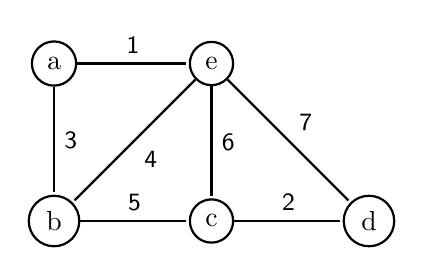
\begin{tikzpicture}[>=stealth',shorten >=1pt,auto,node distance=2cm,
	thick,main node/.style={circle,draw}]
	
	\node[main node] (a) {a};
	\node[main node] (e) [right of=a] {e};
	\node[main node] (b) [below of=a] {b};
	\node[main node] (c) [below of=e] {c};
	\node[main node] (d) [right of=c] {d};
	
	\path[every node/.style={font=\sffamily\small}]
	(a) edge node [] {1} (e)
	(a)	edge node [] {3} (b)
	(e)	edge node [] {4} (b)
	(e)	edge node [] {6} (c)
	(e) edge node [] {7} (d)
	(b) edge node [] {5} (c)
	(c) edge node [] {2} (d);
	\end{tikzpicture}
\end{figure}

\subsubsection*{Sort the edges}
\begin{table}[H]
	\centering
	\begin{tabular}{|c |c |c| c| c| c| c |c|}
		\hline
		Edge	&	(a,e)	&	(c,d)	&	(a,b)	&	(b,e)	&	(b,c)	&	(e,c)	&	(e,d)\\
		\hline
		Weight	&	1		&	2		&	3		&	4		&	5		&	6		&	7\\
		\hline
	\end{tabular}
\end{table}

\subsubsection*{Initial Graph}

\begin{figure}[H]
	\centering
	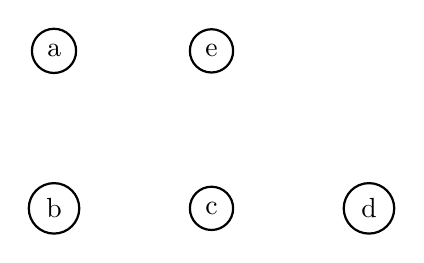
\begin{tikzpicture}[>=stealth',shorten >=1pt,auto,node distance=2cm,
	thick,main node/.style={circle,draw}]
	
	\node[main node] (a) {a};
	\node[main node] (e) [right of=a] {e};
	\node[main node] (b) [below of=a] {b};
	\node[main node] (c) [below of=e] {c};
	\node[main node] (d) [right of=c] {d};
	\end{tikzpicture}
\end{figure}

\subsubsection*{Adding Edge (a,e)}

\begin{figure}[H]
	\centering
	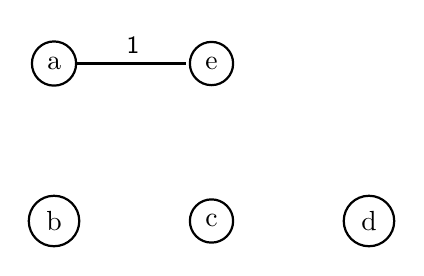
\begin{tikzpicture}[>=stealth',shorten >=1pt,auto,node distance=2cm,
	thick,main node/.style={circle,draw}]
	
	\node[main node] (a) {a};
	\node[main node] (e) [right of=a] {e};
	\node[main node] (b) [below of=a] {b};
	\node[main node] (c) [below of=e] {c};
	\node[main node] (d) [right of=c] {d};
	
	\path[every node/.style={font=\sffamily\small}]
	(a) edge node [] {1} (e);
	\end{tikzpicture}
\end{figure}

\subsubsection*{Adding Edge (c,d)}

\begin{figure}[H]
	\centering
	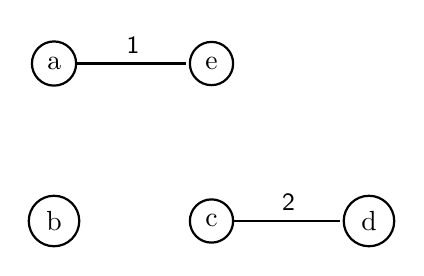
\begin{tikzpicture}[>=stealth',shorten >=1pt,auto,node distance=2cm,
	thick,main node/.style={circle,draw}]
	
	\node[main node] (a) {a};
	\node[main node] (e) [right of=a] {e};
	\node[main node] (b) [below of=a] {b};
	\node[main node] (c) [below of=e] {c};
	\node[main node] (d) [right of=c] {d};
	
	\path[every node/.style={font=\sffamily\small}]
	(a) edge node [] {1} (e)
	(c) edge node [] {2} (d);
	\end{tikzpicture}
\end{figure}

\subsubsection*{Adding Edge (a,b)}

\begin{figure}[H]
	\centering
	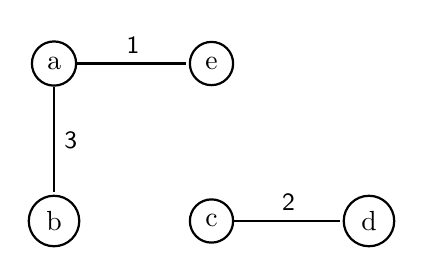
\begin{tikzpicture}[>=stealth',shorten >=1pt,auto,node distance=2cm,
	thick,main node/.style={circle,draw}]
	
	\node[main node] (a) {a};
	\node[main node] (e) [right of=a] {e};
	\node[main node] (b) [below of=a] {b};
	\node[main node] (c) [below of=e] {c};
	\node[main node] (d) [right of=c] {d};
	
	\path[every node/.style={font=\sffamily\small}]
	(a) edge node [] {1} (e)
	(c) edge node [] {2} (d)
	(a) edge node [] {3} (b);
	\end{tikzpicture}
\end{figure}

\subsubsection*{Adding Edge (b,e)}

\begin{figure}[H]
	\centering
	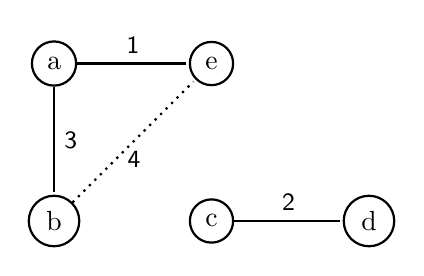
\begin{tikzpicture}[>=stealth',shorten >=1pt,auto,node distance=2cm,
	thick,main node/.style={circle,draw}]
	
	\node[main node] (a) {a};
	\node[main node] (e) [right of=a] {e};
	\node[main node] (b) [below of=a] {b};
	\node[main node] (c) [below of=e] {c};
	\node[main node] (d) [right of=c] {d};
	
	\path[every node/.style={font=\sffamily\small}]
	(a) edge node [] {1} (e)
	(c) edge node [] {2} (d)
	(a) edge node [] {3} (b)
	(b)	edge [dotted] node [below] {4} (e);
	\end{tikzpicture}
	\caption*{Cannot add this edge since it vertex b and vertex e are already in the same tree. }
\end{figure}

\subsubsection*{Adding Edge (b,c)}

\begin{figure}[H]
	\centering
	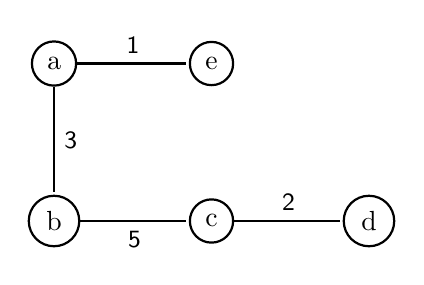
\begin{tikzpicture}[>=stealth',shorten >=1pt,auto,node distance=2cm,
	thick,main node/.style={circle,draw}]
	
	\node[main node] (a) {a};
	\node[main node] (e) [right of=a] {e};
	\node[main node] (b) [below of=a] {b};
	\node[main node] (c) [below of=e] {c};
	\node[main node] (d) [right of=c] {d};
	
	\path[every node/.style={font=\sffamily\small}]
	(a) edge node [] {1} (e)
	(c) edge node [] {2} (d)
	(a) edge node [] {3} (b)
	(b)	edge [] node [below] {5} (c);
	\end{tikzpicture}
	\caption*{All vertices in same tree. Therefore, minimum spanning tree has been derived.}
\end{figure}

\newpage

\section{Minimum Spanning Tree: Prim's Algorithm}

\subsection*{Steps}
\begin{enumerate}
	\item Define an empty tree. 
	\item Select an arbitrary vertex to add to the tree.
	\item Add the least weight edge that connects to the tree.
	\item Repeat until all vertices are connected.
\end{enumerate}

\subsection*{Complexity}
$$
\text{Using adjacency matrix: } O(\vert V \vert^2 )
$$
$$
\text{Using binary heap and adjacency list: } O((\vert V \vert + \vert E \vert) \log(\vert V \vert)) = O(\vert E \vert \log(\vert V \vert))
$$
$$
\text{Using Fibonacci heap and adjacency list: } O(\vert E \vert + \vert V \vert \log(\vert V \vert))
$$

\subsection{Example}
\textbf{Find the minimum spanning tree of the following graph using Prim's algorithm.}

\begin{figure}[H]
	\centering
	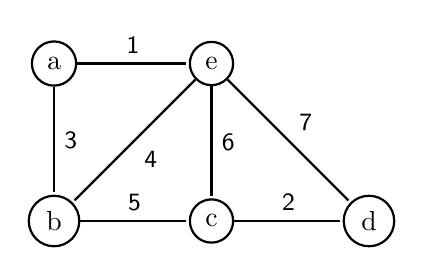
\begin{tikzpicture}[>=stealth',shorten >=1pt,auto,node distance=2cm,
	thick,main node/.style={circle,draw}]
	
	\node[main node] (a) {a};
	\node[main node] (e) [right of=a] {e};
	\node[main node] (b) [below of=a] {b};
	\node[main node] (c) [below of=e] {c};
	\node[main node] (d) [right of=c] {d};
	
	\path[every node/.style={font=\sffamily\small}]
	(a) edge node [] {1} (e)
	(a)	edge node [] {3} (b)
	(e)	edge node [] {4} (b)
	(e)	edge node [] {6} (c)
	(e) edge node [] {7} (d)
	(b) edge node [] {5} (c)
	(c) edge node [] {2} (d);
	\end{tikzpicture}
\end{figure}

\subsubsection*{Initial Tree Starting from Vertex a}

\begin{figure}[H]
	\centering
	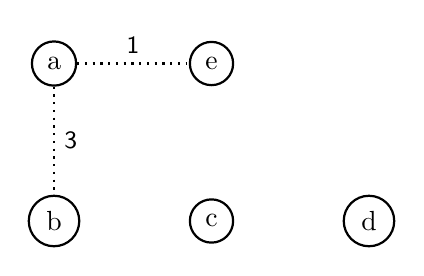
\begin{tikzpicture}[>=stealth',shorten >=1pt,auto,node distance=2cm,
	thick,main node/.style={circle,draw}]
	
	\node[main node] (a) {a};
	\node[main node] (e) [right of=a] {e};
	\node[main node] (b) [below of=a] {b};
	\node[main node] (c) [below of=e] {c};
	\node[main node] (d) [right of=c] {d};
	
	\path[every node/.style={font=\sffamily\small}]
	(a) edge [dotted] node [] {1} (e)
	(a) edge [dotted] node [] {3} (b);
	\end{tikzpicture}
\end{figure}

\subsubsection*{Add edge (a,e)}

\begin{figure}[H]
	\centering
	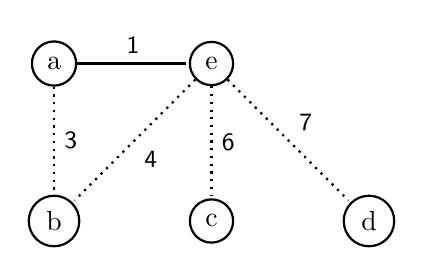
\begin{tikzpicture}[>=stealth',shorten >=1pt,auto,node distance=2cm,
	thick,main node/.style={circle,draw}]
	
	\node[main node] (a) {a};
	\node[main node] (e) [right of=a] {e};
	\node[main node] (b) [below of=a] {b};
	\node[main node] (c) [below of=e] {c};
	\node[main node] (d) [right of=c] {d};
	
	\path[every node/.style={font=\sffamily\small}]
	(a) edge node [] {1} (e)
	(a)	edge [dotted] node [] {3} (b)
	(e)	edge [dotted] node [] {4} (b)
	(e)	edge [dotted] node [] {6} (c)
	(e) edge [dotted] node [] {7} (d);
	\end{tikzpicture}
\end{figure}

\subsubsection*{Add edge (a,b)}

\begin{figure}[H]
	\centering
	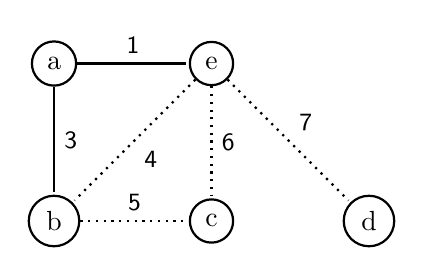
\begin{tikzpicture}[>=stealth',shorten >=1pt,auto,node distance=2cm,
	thick,main node/.style={circle,draw}]
	
	\node[main node] (a) {a};
	\node[main node] (e) [right of=a] {e};
	\node[main node] (b) [below of=a] {b};
	\node[main node] (c) [below of=e] {c};
	\node[main node] (d) [right of=c] {d};
	
	\path[every node/.style={font=\sffamily\small}]
	(a) edge node [] {1} (e)
	(a)	edge [] node [] {3} (b)
	(e)	edge [dotted] node [] {4} (b)
	(e)	edge [dotted] node [] {6} (c)
	(e) edge [dotted] node [] {7} (d)
	(b) edge [dotted] node [] {5} (c);
	\end{tikzpicture}
\end{figure}

\subsubsection*{Add edge (a,b)}

\begin{figure}[H]
	\centering
	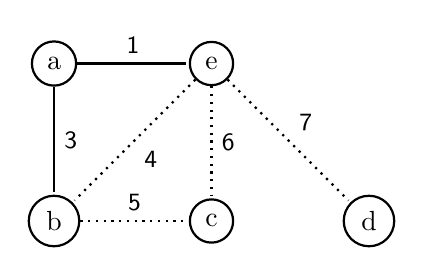
\begin{tikzpicture}[>=stealth',shorten >=1pt,auto,node distance=2cm,
	thick,main node/.style={circle,draw}]
	
	\node[main node] (a) {a};
	\node[main node] (e) [right of=a] {e};
	\node[main node] (b) [below of=a] {b};
	\node[main node] (c) [below of=e] {c};
	\node[main node] (d) [right of=c] {d};
	
	\path[every node/.style={font=\sffamily\small}]
	(a) edge node [] {1} (e)
	(a)	edge [] node [] {3} (b)
	(e)	edge [dotted] node [] {4} (b)
	(e)	edge [dotted] node [] {6} (c)
	(b) edge [dotted] node [] {5} (c)
	(e) edge [dotted] node [] {7} (d);
	\end{tikzpicture}
\end{figure}

\subsubsection*{Add edge (b,e)}

\begin{figure}[H]
	\centering
	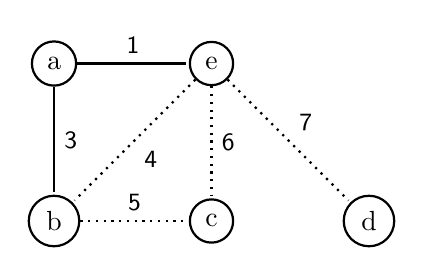
\begin{tikzpicture}[>=stealth',shorten >=1pt,auto,node distance=2cm,
	thick,main node/.style={circle,draw}]
	
	\node[main node] (a) {a};
	\node[main node] (e) [right of=a] {e};
	\node[main node] (b) [below of=a] {b};
	\node[main node] (c) [below of=e] {c};
	\node[main node] (d) [right of=c] {d};
	
	\path[every node/.style={font=\sffamily\small}]
	(a) edge node [] {1} (e)
	(a)	edge [] node [] {3} (b)
	(e)	edge [dotted] node [] {4} (b)
	(e)	edge [dotted] node [] {6} (c)
	(b) edge [dotted] node [] {5} (c)
	(e) edge [dotted] node [] {7} (d);
	\end{tikzpicture}
	\caption*{Cannot edge (b,e) since vertex b and vertex e are in the same tree.}
\end{figure}

\subsubsection*{Add edge (b,c)}

\begin{figure}[H]
	\centering
	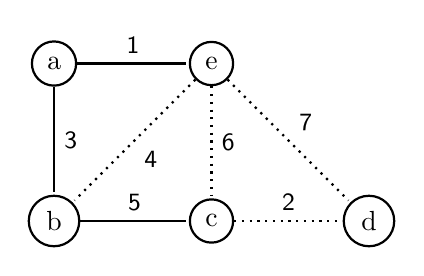
\begin{tikzpicture}[>=stealth',shorten >=1pt,auto,node distance=2cm,
	thick,main node/.style={circle,draw}]
	
	\node[main node] (a) {a};
	\node[main node] (e) [right of=a] {e};
	\node[main node] (b) [below of=a] {b};
	\node[main node] (c) [below of=e] {c};
	\node[main node] (d) [right of=c] {d};
	
	\path[every node/.style={font=\sffamily\small}]
	(a) edge node [] {1} (e)
	(a)	edge [] node [] {3} (b)
	(e)	edge [dotted] node [] {4} (b)
	(e)	edge [dotted] node [] {6} (c)
	(b) edge [] node [] {5} (c)
	(e) edge [dotted] node [] {7} (d)
	(c) edge [dotted] node [] {2} (d);
	\end{tikzpicture}
\end{figure}

\subsubsection*{Add edge (c,d)}

\begin{figure}[H]
	\centering
	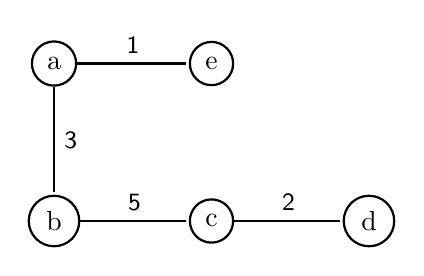
\begin{tikzpicture}[>=stealth',shorten >=1pt,auto,node distance=2cm,
	thick,main node/.style={circle,draw}]
	
	\node[main node] (a) {a};
	\node[main node] (e) [right of=a] {e};
	\node[main node] (b) [below of=a] {b};
	\node[main node] (c) [below of=e] {c};
	\node[main node] (d) [right of=c] {d};
	
	\path[every node/.style={font=\sffamily\small}]
	(a) edge node [] {1} (e)
	(a)	edge [] node [] {3} (b)
	(b) edge [] node [] {5} (c)
	(c) edge [] node [] {2} (d);
	\end{tikzpicture}
	\caption*{All vertices in same tree. Therefore, minimum spanning tree has been derived.}
\end{figure}
\newpage

\section{Case Study: Breadth First Search (BFS)}
\newpage

\section{Case Study: Depth-First Search (DFS)}
\newpage

%
% APPENDIX
%
\appendix
\chapter{Test}
\subsection{Solving Recurrence Relations with Induction}

\subsubsection{Example}
\textbf{Prove that the following systems of equations has the solution $T(n) = n \cdot lg(n)$.}
$$
T(n) \begin{cases}
	2T(\frac{n}{2}) + n, & n = 2^k \mbox{ for } k > 1\\
	2, & n = 2
\end{cases}
$$
\textbf{Basis}
\begin{eqnarray*}
T(2) &=& (2) \cdot lg(2)\\
	&=& 2 \cdot 1\\
	&=& 2
\end{eqnarray*}
\textbf{Inductive Hypothesis}\\
Assume that $T(n) = n \cdot lg(n)$ holds true for all $n = 2^k$.\\\\
\textbf{Inductive Step}
\begin{align*}
T(n)	&=	2T(\frac{n}{2}) + n						&& \text{Base equation}\\
		&= 	2T(\frac{2^{k+1}}{2}) + 2^{k+1}			&& \text{Substitute n with } 2^{k+1}\\
		&= 	2T(2^{k}) + 2^{k+1}						&& \text{Simplify parameters to function T(...)}\\
		&=	2(2^k \cdot lg(2^k)) + 2^{k+1}			&& \text{Inductive hypothesis}\\
		&=	2^{k+1} \left[ lg(2^k) + 1 \right]		&& \text{Distributive property}\\
		&=  2^{k+1} \left[ lg(2^k) + lg(2) \right]  && \text{Logarithmic identity}\\
		&= 	2^{k+1} \cdot lg(2^k \cdot 2)			&& \text{Logarithmic identity}\\
		&=  2^{k+1} \cdot lg(2^{k+1})				&& \text{Exponent property}\\
		&											&& \text{Q.E.D}
\end{align*}

\subsubsection{Example}
\textbf{Prove that the following systems of equations has the solution $T(n) = 2F(n) - 1$ where $F(n) = F(n-1) + F(n-2)$.}
$$
T(n) \begin{cases}
T(n-1) + T(n-2) + 1, & \mbox{if } n \geq 2\\
0, & \mbox{if } n = \{0,1\}
\end{cases}
$$
\textbf{Basis}
\begin{eqnarray*}
	T(0) &=& 1
\end{eqnarray*}
\textbf{Inductive Hypothesis}\\
Assume that $T(n) = F(n) - 1$ is true for all $n = k$.\\
\textbf{Inductive Step}
\begin{align*}
	T(n) 	&= T(n-1) + T(n-2) + 1					&& \text{Base equation}\\
	T(k+1) 	&= T((k+1) - 1) + T((k+1) - 2) + 1 		&& \text{Substitute n with k+1}\\
			&= T(k) + T(k-1) + 1					&& \text{Simplify parameters to function T(...)}\\
			&= (2F(k) - 1) + (2F(k-1) - 1) + 1		&& \text{Inductive hypothesis}\\
			&= 2F(k) + 2F(k-1) - 1					&& \text{Simplify equation}\\
			&= 2(F(k) + F(k-1)) - 1					&& \text{Distributive property}\\
			&= 2(F(k+1)) - 1						&& \text{Definition of function: } F(k+1) = F(k) + F(k-1)\\
			&= 2F(k+1) - 1							&& \text{Simplify}\\
			&										&& \text{Q.E.D}
\end{align*}


\end{document}